\chapter{Results} \label{results}
This chapter will encompass the result of the two ML models for NBRA prediction in Instagram and Flickr media objects as well as the evaluation of the in-situ interviews and the passive observation statistic of NBRAs.
\section{Data-processing} \label{results_dataprocessing}
The following table \ref{tab:data_reduction_values}will provide data-reduction values for each data-source and dataset used. These reductions were the result of the different data-processing steps described in \ref{data_processing} which will be shortly listed again below:
\begin{itemize}
  \item in boundary check
  \item dominant authors exclusion
  \item bulk uploads
\end{itemize}

\begin{table}[ht]
\begin{center}
\caption{Data-reduction according to the different data-sources as a result of data-processing steps}\vspace{1ex}
\label{tab:data_reduction_values}
\begin{tabular}{llccc}\hline
dataset & top authors excluded & bulk threshold & input & output & data-reduction\\ \hline
Instagram Zug & 6 & 6 & 28'246 & 11'777 & 58.3\% \\
Instagram Zurich Uetliberg & 10 & 5 & 74'742 & 68'522 & 8.3\% \\
Instagram Zurich Dolder & 7 & 5 &  206'454 &  191'584 & 7.2\% \\
Flickr Zug & 12 & 7 &  14'236 &  3'790 & 73.4\% \\ 
Foursquare Zug & - & - & 405 & 405 & 0.0\% \\ \hline
\end{tabular}
\end{center}
\end{table}

The noticeably high data-reduction of the Flickr dataset was mostly due to high user upload activity. As seen in figure \ref{img:dominant_users_flickr} a small portion of Flickr-users (authors) uploading up to  1'190 posts since the SMP Flickr was launched in 2005 account for a big share of the entire dataset. As a result to reduce this bias, roughly 5'700 media objects were removed alone in the 'dominant user' data-processing step.\\
Similar graphs to figure \ref{img:dominant_users_flickr} were created for all the datasets according to which the thesis author decided the thresholds in \ref{tab:data_reduction_values} manually. 

\begin{figure}[ht]
   \centering
   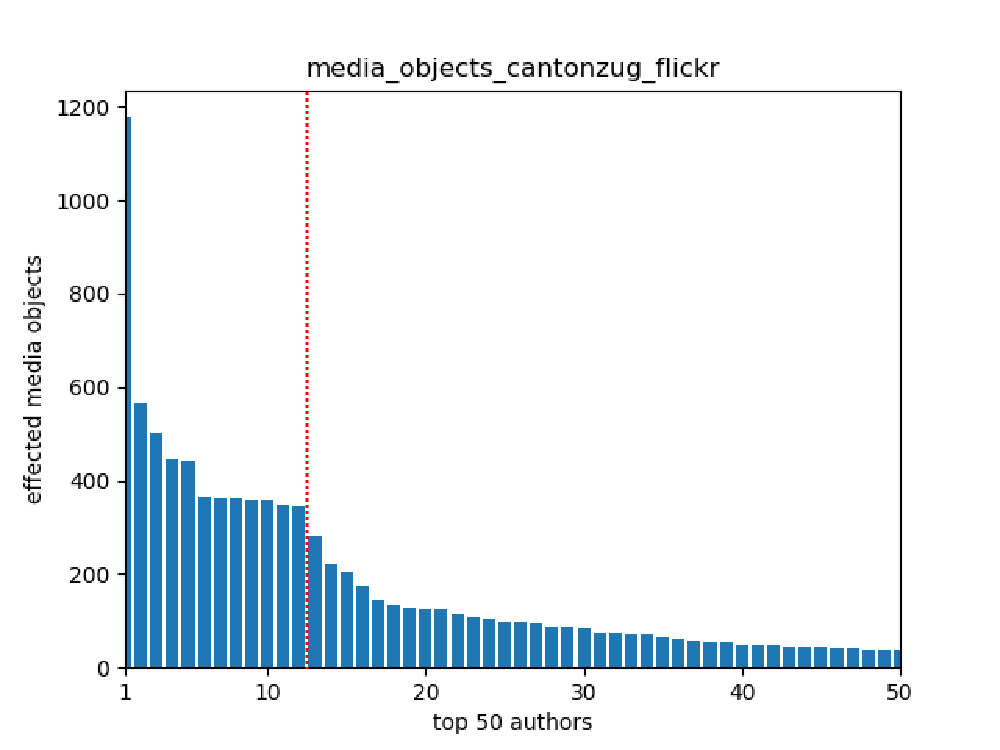
\includegraphics[width=0.75\textwidth]{img/cantonzug_flickr_top50_w_line}
   \caption{The top 12 Flickr authors which account for roughly 5'700 media objects (left to the red line) were excluded from further data-analysis}
   \label{img:dominant_users_flickr}
\end{figure}

\section{Models} \label{results_models}
The following subsections will cover the  performance results of each of the two created models (see chapter \ref{ml_model} that were solely trained on the Instagram Zurich Dolder and Instagram Zurich Uetliberg datasets included in the database table:\\ \texttt{media\_objects\_trainingdata\_instagram} (see figure \ref{database_setup}). For each model the random forest classifier and the linearSVC fitting algorithm was independently tested. The hyperparameters were tuned to yield the best possible average F1-score over all classes excluding the None-class. Simultaneously, the effect of including different amounts of the None-class training's data media objects during model fitting were also tested. These values ranged from 500 to 6’500 with steps of 500.\\
These models were then used to predict the NBRAs contained in the media objects contained in the Instagram database table: \texttt{media\_objects\_unionzug\_instagram} and the \\Flickr database table: \texttt{media\_objects\_cantonzug\_flickr} from the Canton Zug.\\
Each model performed two separate predictions on each of the above mentioned datasets which differed in the final text-string composition that was parsed for prediction. One time the final text-string was constructed by concatenating the processed text-data and the image labels of a given media object. The second time the final text-string only contained the processed text-data.

\subsection{Model 1: untrained on image labels}
The first model (M1) that was trained exclusively on the processed user generated text-data (see chapter \ref{text_processing}). Therefore, it did not include any information about the image and its content. This leads to the model vocabulary potentially missing the associated image labels that the image recognition would yield.

\subsubsection{M1 - Random forest}
The model tuning with the parameter grid visible in figure \ref{fig:randomForest_hyperparameters} resulted in the following best hyper-parameter performing constellation:\\

\begin{table}[ht]
\begin{center}
\caption{Best hyperparameter setting for the random forest algorithm. The parameter descriptions can be found in Chapter \ref{model_setup}}\vspace{1ex}
\label{tab:m1_randomForest_bestParams}
\begin{tabular}{llccc}\hline
k & max\_depth & min\_df & ngram\_range & none\_objects \\ \hline
all & None (no restriction) & 11 & (1, 1) & 3'500 \\ \hline
\end{tabular}
\end{center}
\end{table}

This hyper-parameter setting visible in the table \ref{tab:m1_randomForest_bestParams} allowed for the best model performance with a resulting number of \textbf{727 features}. All scores listed in table \ref{tab:m1_randomForest_bestscores} were rounded to three decimal places and were calculated with the scikit-learn 'weighted' parameter. The 'F1-score'-column refers to the weighted average across all classes whereas the 'F1-score without none class' refers to the weighted average across all classes except the none class.

\begin{table}[ht]
\begin{center}
\caption{M1 random forest performance scores during testing (except accuracy train)}\vspace{1ex}
\label{tab:m1_randomForest_bestscores}
\begin{tabular}{cccccc}\hline
Accuracy train & Accuracy test & Precision & Recall & F1 & F1 (without none class)\\ \hline
0.999 & 0.941 & 0.941 & 0.941 & 0.936 & 0.757 \\ \hline
\end{tabular}
\end{center}
\end{table}

\subsubsection{M1 - LinearSVC}
The model tuning with the parameter grid visible in figure \ref{fig:linearSVC_hyperparameters} resulted in the following best performing hyperparameter constellation:

\begin{table}[ht]
\begin{center}
\caption{Best hyperparameter setting for the linearSVC algorithm. The parameter descriptions can be found in chapter \ref{model_setup}}\vspace{1ex}
\label{tab:m1_linearSVC_bestParams}
\begin{tabular}{llccc}\hline
k & C & min\_df & ngram\_range & none\_objects \\ \hline
all & 1 & 12 & (1, 1) & 3'000 \\ \hline
\end{tabular}
\end{center}
\end{table}

This hyper-parameter setting visible in the table \ref{tab:m1_linearSVC_bestParams} allowed for the best model performance with a resulting number of \textbf{626 features}. All scores listed in table \ref{tab:m1_linearSVC_bestscores} were rounded to three decimal places. The 'F1-score'-column refers to the weighted average1 across all classes whereas the 'F1-score without none class' refers to the weighted average1 across all classes except the none class.

\begin{table}[ht]
\begin{center}
\caption{M1 linearSVC performance scores during testing (except accuracy train)}\vspace{1ex}
\label{tab:m1_linearSVC_bestscores}
\begin{tabular}{cccccc}\hline
Accuracy train & Accuracy test & Precision & Recall & F1 & F1 (without none class)\\ \hline
0.983 & 0.937 & 0.937 & 0.937 & 0.937 & 0.870 \\ \hline
\end{tabular}
\end{center}
\end{table}

\subsection{Model 2: trained on image labels and text-data}
The second model (M2) was trained on the Google Cloud Vision API image labels and the processed user generated text-data (see chapter \ref{text_processing}).

\subsubsection{M2 - Random forest}
The model tuning with the parameter grid visible in figure \ref{fig:randomForest_hyperparameters} resulted in the following best hyper-parameter performing constellation:\\

\begin{table}[ht]
\begin{center}
\caption{Best hyperparameter setting for the random forest algorithm. The parameter descriptions can be found in Chapter \ref{model_setup}}\vspace{1ex}
\label{tab:m2_randomForest_bestParams}
\begin{tabular}{llccc}\hline
k & max\_depth & min\_df & ngram\_range & none\_objects \\ \hline
all & None (no restriction) & 14 & (1, 1) & 400 \\ \hline
\end{tabular}
\end{center}
\end{table}

This hyper-parameter setting visible in the table \ref{tab:m2_randomForest_bestParams} allowed for the best model performance with a resulting number of \textbf{324 features}. All scores listed in table \ref{tab:m2_randomForest_bestscores} were rounded to three decimal places and were calculated with the scikit-learn 'weighted' parameter. The 'F1-score'-column refers to the weighted average across all classes whereas the 'F1-score without none class' refers to the weighted average across all classes except the none class.

\begin{table}[ht]
\begin{center}
\caption{M2 random forest performance scores during testing (except accuracy train)}\vspace{1ex}
\label{tab:m2_randomForest_bestscores}
\begin{tabular}{cccccc}\hline
Accuracy train & Accuracy test & Precision & Recall & F1 & F1 (without none class)\\ \hline
0.998 & 0.892 & 0.903 & 0.901 & 0.892 & 0.745\\ \hline
\end{tabular}
\end{center}
\end{table}

\subsubsection{M2 - LinearSVC}
The model tuning with the parameter grid visible in figure \ref{fig:linearSVC_hyperparameters} resulted in the following best performing hyperparameter constellation:

\begin{table}[ht]
\begin{center}
\caption{Best hyperparameter setting for the linearSVC algorithm. The parameter descriptions can be found in chapter \ref{model_setup}}\vspace{1ex}
\label{tab:m2_linearSVC_bestParams}
\begin{tabular}{llccc}\hline
k & C & min\_df & ngram\_range & none\_objects \\ \hline
all & 1 & 7 & (1, 1) & 700 \\ \hline
\end{tabular}
\end{center}
\end{table}

This hyper-parameter setting visible in the table \ref{tab:m2_linearSVC_bestParams} allowed for the best model performance with a resulting number of \textbf{775 features}. All scores listed in table \ref{tab:m2_linearSVC_bestscores} were rounded to three decimal places. The 'F1-score'-column refers to the weighted average1 across all classes whereas the 'F1-score without none class' refers to the weighted average1 across all classes except the none class.

\begin{table}[ht]
\begin{center}
\caption{M2 linearSVC performance scores during testing (except accuracy train)}\vspace{1ex}
\label{tab:m2_linearSVC_bestscores}
\begin{tabular}{cccccc}\hline
Accuracy train & Accuracy test & Precision & Recall & F1 & F1 (without none class)\\ \hline
0.993 & 0.882 & 0.883 & 0.886 & 0.882 & 0.835 \\ \hline
\end{tabular}
\end{center}
\end{table}

\subsection{Model comparison}
In the following subsections, the above presented models will be thoroughly compared in terms of classification specific performance and hyperparameter behaviour. 

\subsubsection{Hyperparameter constellation}
The effect of different ngram\_range settings in combination with varying C values is illustrated in figure \ref{fig:heatmaps} for M1 and M2 respectively. The red circles indicates the highest F1-score present which corresponds to the best hyperparameter setting of the respective model (see table \ref{tab:m2_linearSVC_bestParams}). It becomes apparent, that the (2, 2) ngram\_range as well as the C value 0.01 underperform across the board. The F1-scores in the heatmaps are not completely identical to the values found in the corresponding model performance tables \ref{tab:m1_linearSVC_bestscores} and \ref{tab:m2_linearSVC_bestscores}. This variation is due to randomisation effects of the none-object selection from the database as well as from the model train and test splits (this is partly taken care of by cross-validation).\\

\begin{figure}[ht]
 \begin{subfigure}{0.5\textwidth}
   \centering
   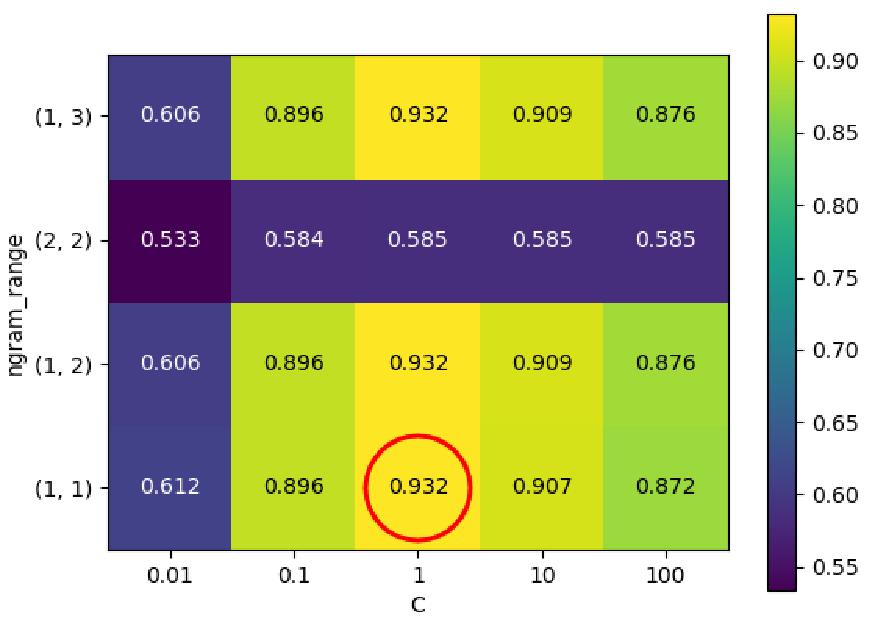
\includegraphics[width=0.9\linewidth]{img/m1_F1_ngram_C_heatmap_w_Circle.pdf}
   \caption{M1 linearSVC}
   \label{fig:m1_heatmap}
\end{subfigure}
\begin{subfigure}{0.5\textwidth}
   \centering
   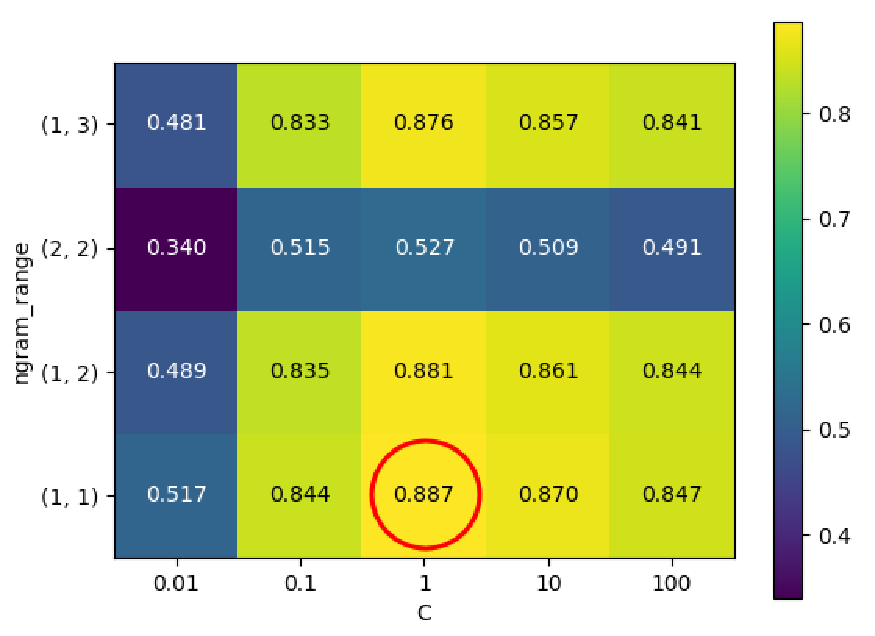
\includegraphics[width=0.9\linewidth]{img/m2_ngram_C_heatmap_new_w_circle.pdf}
   \caption{M2 linearSVC}
   \label{fig:m2_heatmap}
 \end{subfigure}
\caption{These heatmaps shows cross-validated F1-scores dependent on different combinations of the hyper-parameters ngram\_range and C for the model M1 (a) and M2 (b). These graphs were created with the Python library 'mglearn' from \parencite{Guido2016}}
\label{fig:heatmaps}
\end{figure}

\texttt{Remark:} If different hyperparameter settings produce the same model performance (F1-score) than the setting which produces fewer features is prioritised due to better generalisation capabilities. Regarding figure \ref{fig:m1_heatmap} for instance, the n\_gram setting of either (1, 1), (1, 2) or (1, 3) in combination with C = 1 all produce a F1-score of 0.932. (1, 1) has been chosen as best hyperparameter configuration due to the lowest feature count.

\subsubsection{Classification specific F1-scores}

\begin{figure}[ht]
   \centering
   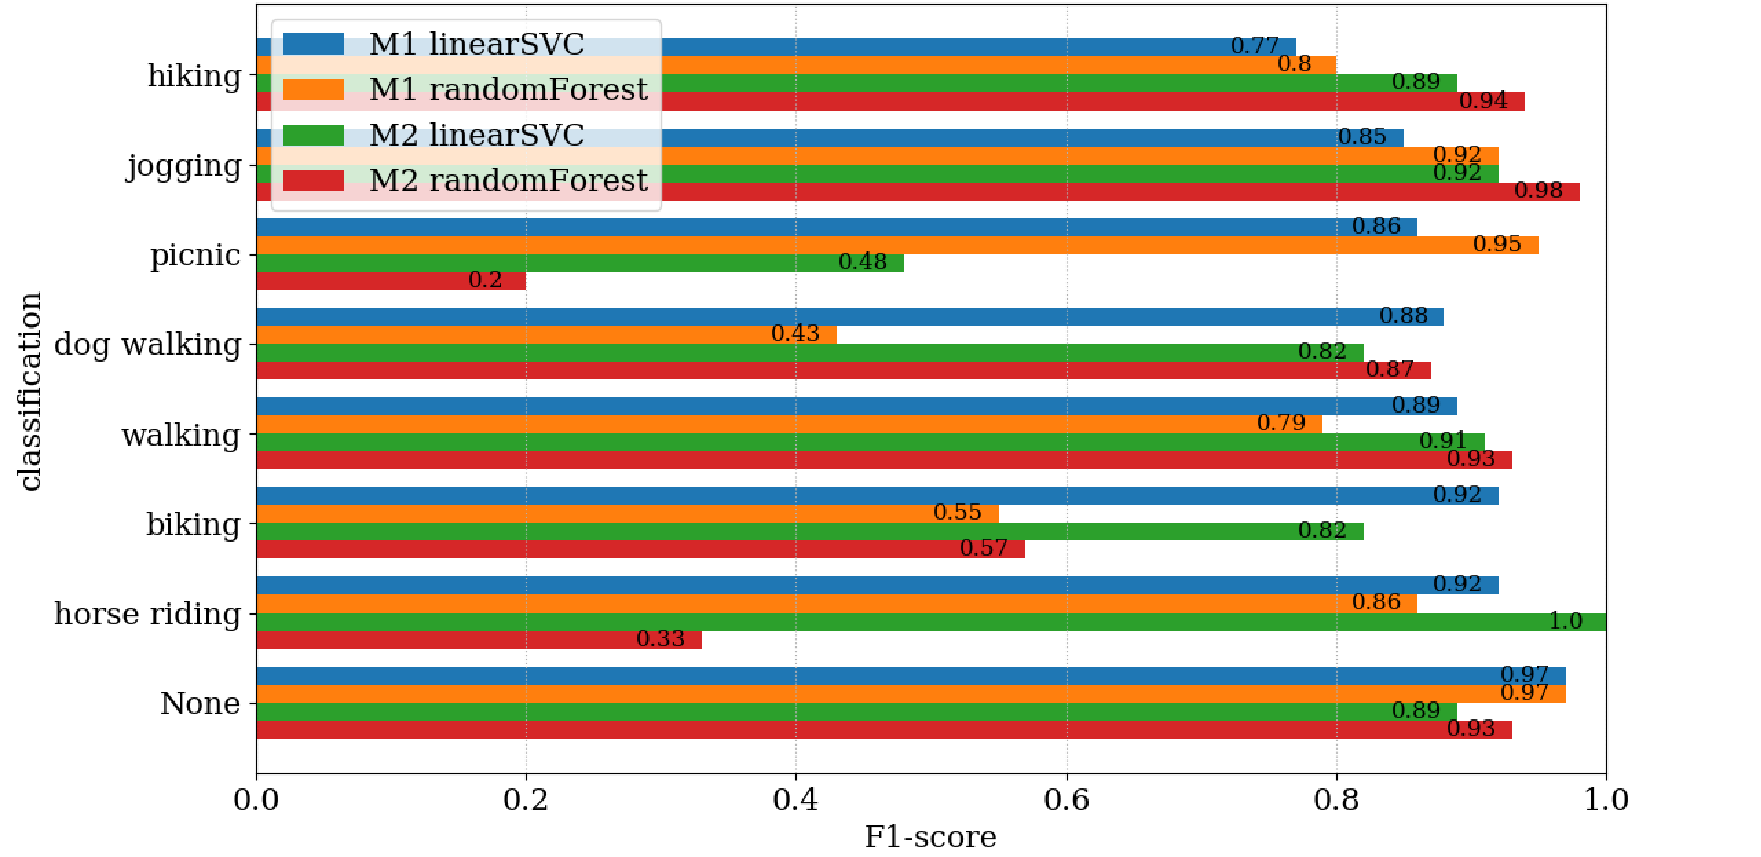
\includegraphics[width=\textwidth]{img/m1_m2_class_f1_scores_bigger_font.pdf}
   \caption{Comparison of the classification specific F1-scores of the linearSVC and random forest fitting algorithm of M1 and M2}
   \label{fig:m1_m2_class_f1_scores}
\end{figure}

\subsubsection{Final model scores}
In the end the model M1 and M2 were trained on the entire training's dataset which resulted in the following final performance scores visible in table \ref{XY}. This step is important to generate a final model that is eventually trained on as much training's data as possible. Keeping a portion of the training's dataset aside for model validation is no longer necessary because the most well performing hyperparameter configuration was already determined before.

\begin{table}[h]
\begin{center}
\caption{M2 linearSVC performance scores during testing (except accuracy train)}\vspace{1ex}
\label{tab:m2_linearSVC_bestscores}
\begin{tabular}{cccccc}\hline
Model & Accuracy & Precision & Recall & F1 & F1 (without none class)\\ \hline
M1 & 0.984 & 0.984 & 0.984 & 0.984 & 0.967 \\
M2 & 0.991 & 0.991 & 0.991 & 0.991 & 0.993 \\ \hline
\end{tabular}
\end{center}
\end{table}

\subsubsection{Precision on unseen data}

\section{spatial distribution of NBRAs}
XXXinsert maps XXX

\section{Language distribution in media objects}


\section{Ground truth evaluation}

\subsection{Passive observation analysis}

\subsection{Interview analysis}
\subsubsection{occasion specific visitation motivations}

\subsubsection{most frequent NBRA’s performed by location}

\subsubsection{Ranking of social media platform usage}

\subsubsection{Relation between age and social media presence}


